\documentclass{article}
\usepackage{tikz}
\usepackage{tikz-network}

\begin{document}


\begin{tikzpicture}
\filldraw (-.2,.2) circle (2pt) (.2,.2) circle (2pt);
\draw (0,0) circle (5mm) ;
\end{tikzpicture}


{
.\newline\newline\newline
}

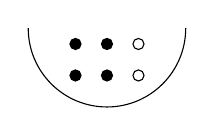
\begin{tikzpicture}
\draw (0,0) arc (180:360:1) ;
\filldraw (.6,-.2) circle (2pt) (.6,-.6) circle (2pt);
\filldraw (1,-.2) circle (2pt) (1,-.6) circle (2pt);
\draw (1.4,-.2) circle (2pt) (1.4,-.6) circle (2pt);
\end{tikzpicture}


{
.\newline\newline\newline
}


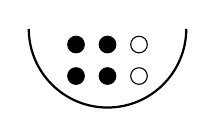
\begin{tikzpicture}
\draw[thick]  (0,0) arc (180:360:1) ;
\filldraw (.6,-.2) circle (3pt) (.6,-.6) circle (3pt);
\filldraw (1,-.2) circle (3pt) (1,-.6) circle (3pt);
\draw (1.4,-.2) circle (3pt) (1.4,-.6) circle (3pt);
\end{tikzpicture}


{
.\newline\newline\newline
}



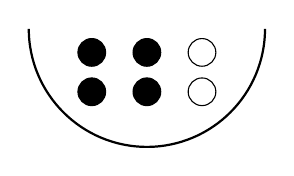
\begin{tikzpicture}
\draw[thick]  (0,0) arc (180:360:1.5) ;
\filldraw (.8,-.3) circle (5pt) (.8,-.8) circle (5pt);
\filldraw (1.5,-.3) circle (5pt) (1.5,-.8) circle (5pt);
\draw (2.2,-.3) circle (5pt) (2.2,-.8) circle (5pt);
\end{tikzpicture}


{
.\newline\newline\newline
}



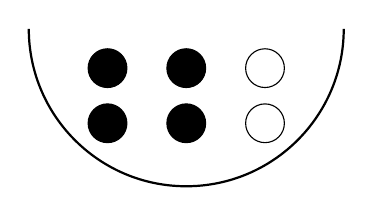
\begin{tikzpicture}
\draw[thick]  (0,0) arc (180:360:2) ;
\filldraw (1,-.5) circle (7pt) (1,-1.2) circle (7pt);
\filldraw (2,-.5) circle (7pt) (2,-1.2) circle (7pt);
\draw (3,-.5) circle (7pt) (3,-1.2) circle (7pt);
\end{tikzpicture}


{
.\newline\newline\newline
}


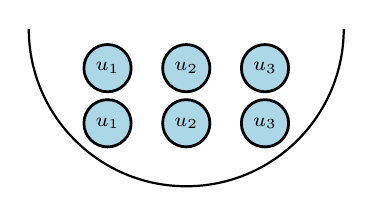
\begin{tikzpicture}
\draw[thick]  (0,0) arc (180:360:2) ;
\Vertex[x=1,y=-.5,label=$u_1$]{A1}
\Vertex[x=1,y=-1.2,label=$u_1$]{A2}

\Vertex[x=2,y=-.5,label=$u_2$]{B1}
\Vertex[x=2,y=-1.2,label=$u_2$]{B2}

\Vertex[x=3,y=-.5,label=$u_3$]{C1}
\Vertex[x=3,y=-1.2,label=$u_3$]{C2}
\end{tikzpicture}


{
.\newline\newline\newline
}



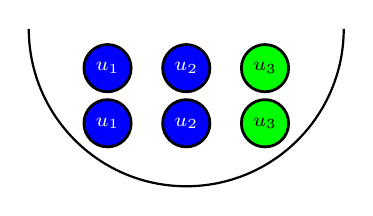
\begin{tikzpicture}
\draw[thick]  (0,0) arc (180:360:2) ;
\Vertex[x=1,y=-.5,label=$u_1$,color=blue,fontcolor=white]{A1}
\Vertex[x=1,y=-1.2,label=$u_1$,color=blue,fontcolor=white]{A2}

\Vertex[x=2,y=-.5,label=$u_2$,color=blue,fontcolor=white]{B1}
\Vertex[x=2,y=-1.2,label=$u_2$,color=blue,fontcolor=white]{B2}

\Vertex[x=3,y=-.5,label=$u_3$,color=green]{C1}
\Vertex[x=3,y=-1.2,label=$u_3$,color=green]{C2}
\end{tikzpicture}


{
.\newline\newline\newline
}



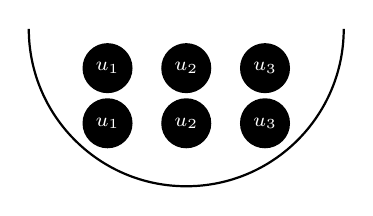
\begin{tikzpicture}
\draw[thick]  (0,0) arc (180:360:2) ;
\Vertex[x=1,y=-.5,label=$u_1$,color=black,fontcolor=white]{A1}
\Vertex[x=1,y=-1.2,label=$u_1$,color=black,fontcolor=white]{A2}

\Vertex[x=2,y=-.5,label=$u_2$,color=black,fontcolor=white]{B1}
\Vertex[x=2,y=-1.2,label=$u_2$,color=black,fontcolor=white]{B2}

\Vertex[x=3,y=-.5,label=$u_3$,color=black,fontcolor=white]{C1}
\Vertex[x=3,y=-1.2,label=$u_3$,color=black,fontcolor=white]{C2}
\end{tikzpicture}


{
.\newline\newline\newline
}




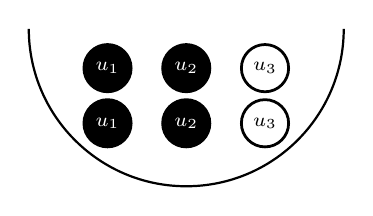
\begin{tikzpicture}
\draw[thick]  (0,0) arc (180:360:2) ;
\Vertex[x=1,y=-.5,label=$u_1$,color=black,fontcolor=white]{A1}
\Vertex[x=1,y=-1.2,label=$u_1$,color=black,fontcolor=white]{A2}

\Vertex[x=2,y=-.5,label=$u_2$,color=black,fontcolor=white]{B1}
\Vertex[x=2,y=-1.2,label=$u_2$,color=black,fontcolor=white]{B2}

\Vertex[x=3,y=-.5,label=$u_3$,color=white,fontcolor=black]{C1}
\Vertex[x=3,y=-1.2,label=$u_3$,color=white,fontcolor=black]{C2}
\end{tikzpicture}


{
.\newline\newline\newline
}




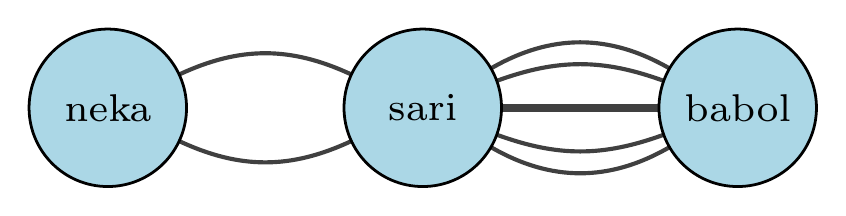
\begin{tikzpicture}
\Vertex[x=0,label=neka,size=2,fontscale=2]{A} 
\Vertex[x=4,label=sari,size=2,fontscale=2]{B}
\Vertex[x=8,label=babol,size=2,fontscale=2]{C}

\Edge[bend=25](A)(B)
\Edge[bend=-25](A)(B)

\Edge[bend=30](B)(C)
\Edge[bend=20](B)(C)
\Edge[bend=0,lw=3pt](B)(C)
\Edge[bend=-20](B)(C)
\Edge[bend=-30](B)(C)

\end{tikzpicture}



{
.\newline\newline\newline
}



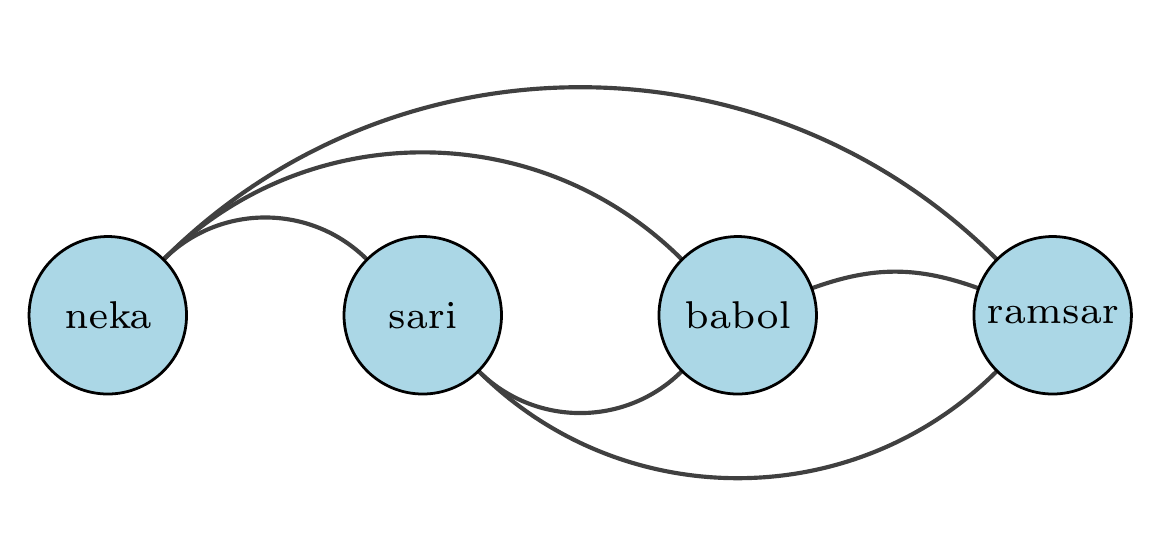
\begin{tikzpicture}
\Vertex[x=0,label=neka,size=2,fontscale=2]{A} 
\Vertex[x=4,label=sari,size=2,fontscale=2]{B}
\Vertex[x=8,label=babol,size=2,fontscale=2]{C}
\Vertex[x=12,label=ramsar,size=2,fontscale=2]{D}

\Edge[bend=45](A)(B)
\Edge[bend=45](A)(C)
\Edge[bend=45](A)(D)

\Edge[bend=-45](B)(C)
\Edge[bend=-45](B)(D)
%\Edge[bend=0,lw=3pt](B)(C)

\Edge[bend=20](C)(D)


\end{tikzpicture}




{
.\newline\newline\newline
}





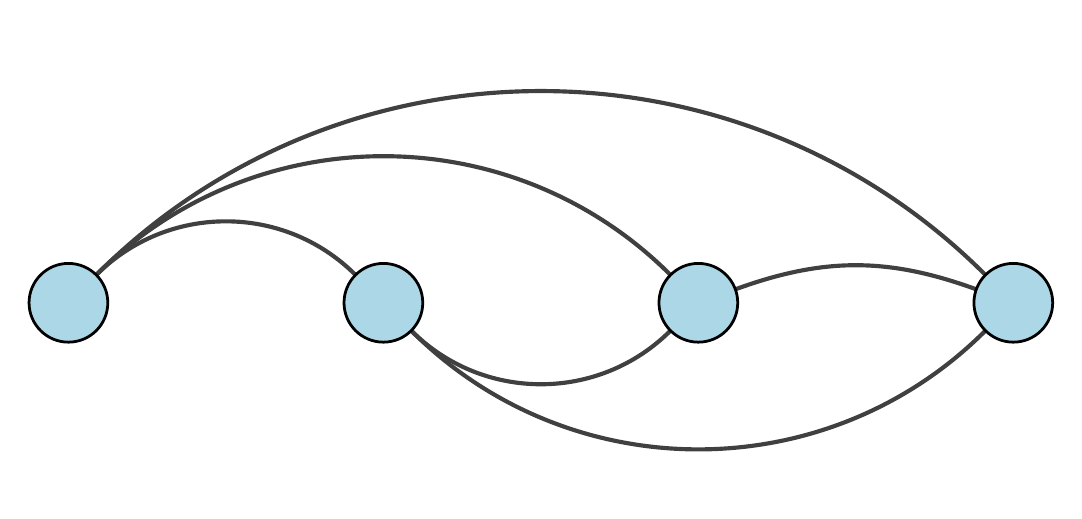
\begin{tikzpicture}
\Vertex[x=0,size=1,fontscale=2]{A} 
\Vertex[x=4,size=1,fontscale=2]{B}
\Vertex[x=8,size=1,fontscale=2]{C}
\Vertex[x=12,size=1,fontscale=2]{D}

\Edge[bend=45](A)(B)
\Edge[bend=45](A)(C)
\Edge[bend=45](A)(D)

\Edge[bend=-45](B)(C)
\Edge[bend=-45](B)(D)
%\Edge[bend=0,lw=3pt](B)(C)

\Edge[bend=20](C)(D)

\end{tikzpicture}




{
.\newline\newline\newline
}



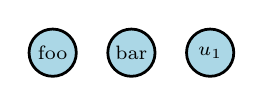
\begin{tikzpicture}
\Vertex[label=foo]{A}
\Vertex[x=1,label=bar]{B}
\Vertex[x=2,label=$u_1$]{C}
\end{tikzpicture}



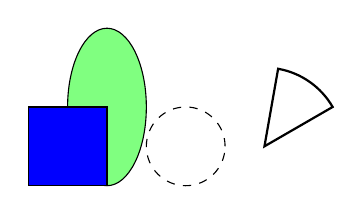
\begin{tikzpicture}
\draw[style=dashed] (2,.5) circle (0.5);
\draw[fill=green!50] (1,1)
ellipse (.5 and 1);
\draw[fill=blue] (0,0) rectangle (1,1);
\draw[style=thick]
(3,.5) -- +(30:1) arc(30:80:1) -- cycle;
\end{tikzpicture}




\setlength{\unitlength}{1mm}
\begin{picture}(60, 40)

\put(15,10){\circle{1}}
\put(20,10){\circle{2}}
\put(25,10){\circle{3}}
\put(30,10){\circle{4}}
\put(35,10){\circle{5}}

\put(15,20){\circle*{1}}
\put(20,20){\circle*{2}}
\put(25,20){\circle*{3}}
\put(30,20){\circle*{4}}
\put(35,20){\circle*{5}}

\end{picture}



\begin{tikzpicture}(60, 40)
 \draw[red] (0,0) arc (30:60:3);
\end{tikzpicture}



\begin{tikzpicture}(60, 40)
 \draw[red] (0,0) arc (0:180:3);
\end{tikzpicture}


{
.\newline\newline
}


\begin{tikzpicture}
 \draw[red] (0,0) arc (180:360:3);
 \put(15,20){\circle*{1}}
\put(20,20){\circle*{2}}
\put(25,20){\circle*{3}}
\put(30,20){\circle*{4}}
\put(35,20){\circle*{5}}
\end{tikzpicture}




\end{document}